\documentclass[10pt]{article}\usepackage[]{graphicx}\usepackage[]{color}
%% maxwidth is the original width if it is less than linewidth
%% otherwise use linewidth (to make sure the graphics do not exceed the margin)
\makeatletter
\def\maxwidth{ %
  \ifdim\Gin@nat@width>\linewidth
    \linewidth
  \else
    \Gin@nat@width
  \fi
}
\makeatother

\definecolor{fgcolor}{rgb}{0.345, 0.345, 0.345}
\newcommand{\hlnum}[1]{\textcolor[rgb]{0.686,0.059,0.569}{#1}}%
\newcommand{\hlstr}[1]{\textcolor[rgb]{0.192,0.494,0.8}{#1}}%
\newcommand{\hlcom}[1]{\textcolor[rgb]{0.678,0.584,0.686}{\textit{#1}}}%
\newcommand{\hlopt}[1]{\textcolor[rgb]{0,0,0}{#1}}%
\newcommand{\hlstd}[1]{\textcolor[rgb]{0.345,0.345,0.345}{#1}}%
\newcommand{\hlkwa}[1]{\textcolor[rgb]{0.161,0.373,0.58}{\textbf{#1}}}%
\newcommand{\hlkwb}[1]{\textcolor[rgb]{0.69,0.353,0.396}{#1}}%
\newcommand{\hlkwc}[1]{\textcolor[rgb]{0.333,0.667,0.333}{#1}}%
\newcommand{\hlkwd}[1]{\textcolor[rgb]{0.737,0.353,0.396}{\textbf{#1}}}%

\usepackage{framed}
\makeatletter
\newenvironment{kframe}{%
 \def\at@end@of@kframe{}%
 \ifinner\ifhmode%
  \def\at@end@of@kframe{\end{minipage}}%
  \begin{minipage}{\columnwidth}%
 \fi\fi%
 \def\FrameCommand##1{\hskip\@totalleftmargin \hskip-\fboxsep
 \colorbox{shadecolor}{##1}\hskip-\fboxsep
     % There is no \\@totalrightmargin, so:
     \hskip-\linewidth \hskip-\@totalleftmargin \hskip\columnwidth}%
 \MakeFramed {\advance\hsize-\width
   \@totalleftmargin\z@ \linewidth\hsize
   \@setminipage}}%
 {\par\unskip\endMakeFramed%
 \at@end@of@kframe}
\makeatother

\definecolor{shadecolor}{rgb}{.97, .97, .97}
\definecolor{messagecolor}{rgb}{0, 0, 0}
\definecolor{warningcolor}{rgb}{1, 0, 1}
\definecolor{errorcolor}{rgb}{1, 0, 0}
\newenvironment{knitrout}{}{} % an empty environment to be redefined in TeX

\usepackage{alltt}

\usepackage{amsmath,epsfig,fullpage,hyperref}%psfig,pstricks,
\parindent 0in
\usepackage[latin1]{inputenc} % LaTeX, comprends les accents !
\usepackage[T1]{fontenc}      % Police contenant les caract?res fran?ais
\usepackage{geometry}         % D?finir les marges
%\usepackage[francais]{babel}  % Placez ici une liste de langues, la
%\pagestyle{headings}        % Pour mettre des ent?tes avec les titres

%\bibliographystyle{frplain}
%\bibliography{myDatabase}
\newcommand{\Robject}[1]{{\texttt{#1}}}
\newcommand{\Rfunction}[1]{{\texttt{#1}}}
\newcommand{\Rpackage}[1]{{\textit{#1}}}
\AtBeginDocument{
        \def\labelitemi{\textbullet}
}
\usepackage{/usr/local/lib/R/share/texmf/Sweave}
\SweaveOpts{prefix.string=graphics/plot}
\IfFileExists{upquote.sty}{\usepackage{upquote}}{}
\begin{document}


\title{\bf R language: A quick tutorial}
\author{Denis Puthier }
\maketitle

\begin{center}
Laboratoire INSERM TAGC/ERM206, Parc Scientifique de Luminy case 928,13288 MARSEILLE cedex 09, FRANCE.
\end{center}

\tableofcontents
\newpage

This tutorial is just a brief tour of the language capabilities and  is intented to give some clues to begin with the R programming language. For a more detailled overview see "R for beginners" (E. Paradis, http://cran.r-project.org/doc/contrib/Paradis-rdebuts\_en.pdf)
\bigskip


\section{Basic aspects of the language.}




R is an object-oriented programming language. You can easily create basic objects of class \Rfunction{vector}, \Rfunction{matrix},
\Rfunction{data.frame}, \Rfunction{list}, \Rfunction{factor},... \medskip

A vector \textit{x} that contains one value.


\begin{knitrout}
\definecolor{shadecolor}{rgb}{0.969, 0.969, 0.969}\color{fgcolor}\begin{kframe}
\begin{alltt}
\hlstd{x} \hlkwb{<-} \hlnum{15}
\end{alltt}
\end{kframe}
\end{knitrout}


\medskip
You can see the content of \textit{x} by simply calling it.

\begin{knitrout}
\definecolor{shadecolor}{rgb}{0.969, 0.969, 0.969}\color{fgcolor}\begin{kframe}
\begin{alltt}
\hlstd{x}
\end{alltt}
\begin{verbatim}
## [1] 15
\end{verbatim}
\end{kframe}
\end{knitrout}

\medskip

Alternatively, you can use the "=" operator. However "<-" is most generally prefered.

\begin{knitrout}
\definecolor{shadecolor}{rgb}{0.969, 0.969, 0.969}\color{fgcolor}\begin{kframe}
\begin{alltt}
\hlstd{x} \hlkwb{=} \hlnum{22}
\hlstd{x}
\end{alltt}
\begin{verbatim}
## [1] 22
\end{verbatim}
\end{kframe}
\end{knitrout}
\medskip


You can add comment by starting a line with a hash (\#). In this case the code at the right of the hash won't be interpreted.

\begin{knitrout}
\definecolor{shadecolor}{rgb}{0.969, 0.969, 0.969}\color{fgcolor}\begin{kframe}
\begin{alltt}
\hlcom{#x <-  57}
\hlstd{x}
\end{alltt}
\begin{verbatim}
## [1] 22
\end{verbatim}
\end{kframe}
\end{knitrout}


\begin{knitrout}
\definecolor{shadecolor}{rgb}{0.969, 0.969, 0.969}\color{fgcolor}\begin{kframe}
\begin{alltt}
\hlstd{x}
\end{alltt}
\begin{verbatim}
## [1] 22
\end{verbatim}
\end{kframe}
\end{knitrout}
\medskip

Instructions can be separated by semi-colons (;) or new-line.

\begin{knitrout}
\definecolor{shadecolor}{rgb}{0.969, 0.969, 0.969}\color{fgcolor}\begin{kframe}
\begin{alltt}
\hlstd{x} \hlkwb{<-} \hlnum{12}\hlstd{; y} \hlkwb{<-} \hlnum{13}
\hlstd{x;y}
\end{alltt}
\begin{verbatim}
## [1] 12
## [1] 13
\end{verbatim}
\end{kframe}
\end{knitrout}


\medskip

Once values are assigned to an object, R will store this object in the memory (RAM). Previously created objects can be \textbf{l}i\textbf{s}ted using the \Rfunction{ls} function.
%code 7
\begin{knitrout}
\definecolor{shadecolor}{rgb}{0.969, 0.969, 0.969}\color{fgcolor}\begin{kframe}
\begin{alltt}
\hlkwd{ls}\hlstd{()}
\end{alltt}
\begin{verbatim}
## [1] "x" "y"
\end{verbatim}
\end{kframe}
\end{knitrout}
\medskip

Object can be deleted using the \Rfunction{rm} (\textbf{r}e\textbf{m}ove) function.
\begin{knitrout}
\definecolor{shadecolor}{rgb}{0.969, 0.969, 0.969}\color{fgcolor}\begin{kframe}
\begin{alltt}
\hlkwd{rm}\hlstd{(x)}
\hlkwd{rm}\hlstd{(y)}
\hlkwd{ls}\hlstd{()}
\end{alltt}
\begin{verbatim}
## character(0)
\end{verbatim}
\end{kframe}
\end{knitrout}

 \medskip

\section{Syntax for calling Functions.}

In the above section we have created vectors containing  numeric data. We have also used functions (\Rfunction{ls} and \Rfunction{rm}). We can use numerous functions to perform specific tasks. When calling a function, we will use this generic syntax:

\begin{center}
\begin{Sinput}
 - NameOfTheFunction(arg1= a, arg2= b,...)
\end{Sinput}
\end{center}
\medskip
arg1 et arg2 (...) : arguments of the function.\medskip
a and b : The objects that will be passed to the function.
\medskip

To access the documentation of a given function, use the \Rfunction{help} function (or the question mark). The documentation gives you an overview of the function (usage, arguments name and class, returned values and examples). For instance to get information about the \Rfunction{substr} function (used to extract part of a character string) use one of the following instructions:

\begin{Soutput}
> help(substr) # or ?substr
\end{Soutput}

\begin{scriptsize}
\begin{Soutput}
substr                 package:base                 R Documentation

Substrings of a Character Vector

Description:

     Extract or replace substrings in a character vector.

Usage:

     substr(x, start, stop)
     substring(text, first, last = 1000000)
     substr(x, start, stop) <- value
     substring(text, first, last = 1000000) <- value

Arguments:

 x, text: a character vector.

start, first: integer. The first element to be replaced.

stop, last: integer. The last element to be replaced.

   value: a character vector, recycled if necessary.

Details:

     'substring' is compatible with S, with 'first' and 'last' instead
     of 'start' and 'stop'. For vector arguments, it expands the
     arguments cyclically to the length of the longest _provided_ none
     are of zero length.

     When extracting, if 'start' is larger than the string length then
     '""' is returned.

     For the extraction functions, 'x' or 'text' will be converted to a
     character vector by 'as.character' if it is not already one.

     For the replacement functions, if 'start' is larger than the
     string length then no replacement is done.  If the portion to be
     replaced is longer than the replacement string, then only the
     portion the length of the string is replaced.

     If any argument is an 'NA' element, the corresponding element of
     the answer is 'NA'.

Value:

     For 'substr', a character vector of the same length and with the
     same attributes as 'x' (after possible coercion).

     For 'substring', a character vector of length the longest of the
     arguments.  This will have names taken from 'x' (if it has any
     after coercion, repeated as needed), and other attributes copied
     from 'x' if it is the longest of the arguments).

Note:

     The S4 version of 'substring<-' ignores 'last'; this version does
     not.

     These functions are often used with 'nchar' to truncate a display.
      That does not really work (you want to limit the width, not the
     number of characters, so it would be better to use 'strtrim'), but
     at least make sure you use 'nchar(type="c")'.

References:

     Becker, R. A., Chambers, J. M. and Wilks, A. R. (1988) _The New S
     Language_. Wadsworth & Brooks/Cole. ('substring'.)

See Also:

     'strsplit', 'paste', 'nchar'.

Examples:

     substr("abcdef",2,4)
     substring("abcdef",1:6,1:6)
     ## strsplit is more efficient ...

     substr(rep("abcdef",4),1:4,4:5)
     x <- c("asfef", "qwerty", "yuiop[", "b", "stuff.blah.yech")
     substr(x, 2, 5)
     substring(x, 2, 4:6)

     substring(x, 2) <- c("..", "+++")
     x
\end{Soutput}
\end{scriptsize}
\medskip
When calling a function, the name of the arguments can be omitted if they are placed as expected. For instance if one wants to extract character 2 to 4 in the string "microarray":

\begin{knitrout}
\definecolor{shadecolor}{rgb}{0.969, 0.969, 0.969}\color{fgcolor}\begin{kframe}
\begin{alltt}
\hlkwd{substr}\hlstd{(}\hlstr{"microarray"}\hlstd{,} \hlnum{2}\hlstd{,}\hlnum{4}\hlstd{)}
\end{alltt}
\begin{verbatim}
## [1] "icr"
\end{verbatim}
\end{kframe}
\end{knitrout}
\medskip
If the  arguments are not in the expected order their names are mandatory (note that, for convenience, they can be abbreviated but the abbreviation used should be unambiguous):


\begin{Soutput}
> substr(2,4,"microarray")                    # arguments are misplaced
[1] NA
Warning message:
In substr(2, 4, "microarray") :
  NAs introduits lors de la conversion automatique
\end{Soutput}

\begin{knitrout}
\definecolor{shadecolor}{rgb}{0.969, 0.969, 0.969}\color{fgcolor}\begin{kframe}
\begin{alltt}
\hlkwd{substr}\hlstd{(}\hlkwc{start}\hlstd{=}\hlnum{2}\hlstd{,}\hlkwc{stop}\hlstd{=}\hlnum{4}\hlstd{,}\hlkwc{x}\hlstd{=}\hlstr{"microarray"}\hlstd{)} \hlcom{# works}
\end{alltt}
\begin{verbatim}
## [1] "icr"
\end{verbatim}
\end{kframe}
\end{knitrout}
\begin{Soutput}
> substr(st=2,st=4,x="microarray")            #ambiguous
Erreur dans substr(st = 2, st = 4, x = "microarray") :
  argument formel "start" correspondant ? plusieurs arguments fournis
\end{Soutput}
\medskip


\section{Modes. Functions for creating vectors.}
\subsection{Modes}
A vector can contain several variables of the same mode. Most frequently, the mode will be one of: "numeric", "character" or "logical".
\subsection{Functions and operators for creating vectors.}
\paragraph{The function \Rfunction{c}}
The function \Rfunction{c} is used to \textbf{c}ombine values into a vector.


\begin{knitrout}
\definecolor{shadecolor}{rgb}{0.969, 0.969, 0.969}\color{fgcolor}\begin{kframe}
\begin{alltt}
\hlstd{mic} \hlkwb{<-} \hlkwd{c}\hlstd{(}\hlstr{"Agilent"}\hlstd{,} \hlstr{"Affy"}\hlstd{)}       \hlcom{# A character vector}
\hlstd{mic}
\end{alltt}
\begin{verbatim}
## [1] "Agilent" "Affy"
\end{verbatim}
\begin{alltt}
\hlkwd{is}\hlstd{(mic)}
\end{alltt}
\begin{verbatim}
## [1] "character"           "vector"              "data.frameRowLabels"
## [4] "SuperClassMethod"
\end{verbatim}
\begin{alltt}
\hlstd{num} \hlkwb{<-} \hlkwd{c}\hlstd{(}\hlnum{1}\hlstd{,}\hlnum{2}\hlstd{,}\hlnum{3}\hlstd{)}                   \hlcom{# A numeric vector}
\hlstd{num}
\end{alltt}
\begin{verbatim}
## [1] 1 2 3
\end{verbatim}
\begin{alltt}
\hlkwd{is}\hlstd{(num)}
\end{alltt}
\begin{verbatim}
## [1] "numeric" "vector"
\end{verbatim}
\begin{alltt}
\hlstd{bool} \hlkwb{<-} \hlkwd{c}\hlstd{(T,F,T)}                  \hlcom{# A logical vector}
\hlstd{bool}
\end{alltt}
\begin{verbatim}
## [1]  TRUE FALSE  TRUE
\end{verbatim}
\begin{alltt}
\hlkwd{is}\hlstd{(bool)}
\end{alltt}
\begin{verbatim}
## [1] "logical" "vector"
\end{verbatim}
\begin{alltt}
\hlstd{num} \hlopt{>} \hlnum{1.5}                          \hlcom{# Also returns a logical vector}
\end{alltt}
\begin{verbatim}
## [1] FALSE  TRUE  TRUE
\end{verbatim}
\end{kframe}
\end{knitrout}
\medskip
\paragraph{The operator ":"}
This operator generates a sequence from 'from' to 'to' in steps of '1' .
For numeric arguments 'from:to' is equivalent to 'seq(from, to)'.

\begin{knitrout}
\definecolor{shadecolor}{rgb}{0.969, 0.969, 0.969}\color{fgcolor}\begin{kframe}
\begin{alltt}
\hlnum{1}\hlopt{:}\hlnum{3}
\end{alltt}
\begin{verbatim}
## [1] 1 2 3
\end{verbatim}
\begin{alltt}
\hlkwd{seq}\hlstd{(}\hlnum{3}\hlstd{,} \hlnum{1}\hlstd{)}
\end{alltt}
\begin{verbatim}
## [1] 3 2 1
\end{verbatim}
\begin{alltt}
\hlnum{3}\hlopt{:}\hlnum{1}                   \hlcom{# Values in decreasing order}
\end{alltt}
\begin{verbatim}
## [1] 3 2 1
\end{verbatim}
\end{kframe}
\end{knitrout}
\medskip
\paragraph{Functions \Rfunction{rep}, \Rfunction{seq}}
The \Rfunction{rep} function \textbf{rep}eats a value as many times as requested.
\begin{knitrout}
\definecolor{shadecolor}{rgb}{0.969, 0.969, 0.969}\color{fgcolor}\begin{kframe}
\begin{alltt}
\hlkwd{rep}\hlstd{(}\hlnum{3}\hlstd{,}\hlnum{5}\hlstd{)}
\end{alltt}
\begin{verbatim}
## [1] 3 3 3 3 3
\end{verbatim}
\end{kframe}
\end{knitrout}

The \Rfunction{seq} function is used to create numeric \textbf{seq}uence.

\begin{knitrout}
\definecolor{shadecolor}{rgb}{0.969, 0.969, 0.969}\color{fgcolor}\begin{kframe}
\begin{alltt}
\hlkwd{seq}\hlstd{(}\hlnum{0}\hlstd{,}\hlnum{10}\hlstd{,}\hlkwc{by}\hlstd{=}\hlnum{2}\hlstd{)}
\end{alltt}
\begin{verbatim}
## [1]  0  2  4  6  8 10
\end{verbatim}
\begin{alltt}
\hlkwd{seq}\hlstd{(}\hlnum{0}\hlstd{,}\hlnum{10}\hlstd{,}\hlkwc{length.out}\hlstd{=}\hlnum{3}\hlstd{)}
\end{alltt}
\begin{verbatim}
## [1]  0  5 10
\end{verbatim}
\end{kframe}
\end{knitrout}
\medskip
\paragraph{Functions to generate random number}

the \Rfunction{rnorm} function is used to generate normally distributed values with mean equal to 'mean' (default 0) and standard deviation equal to 'sd' (default 1).
\begin{knitrout}
\definecolor{shadecolor}{rgb}{0.969, 0.969, 0.969}\color{fgcolor}\begin{kframe}
\begin{alltt}
\hlstd{x} \hlkwb{<-} \hlkwd{rnorm}\hlstd{(}\hlnum{1000}\hlstd{,}\hlkwc{mean}\hlstd{=}\hlnum{2}\hlstd{,}\hlkwc{sd}\hlstd{=}\hlnum{2}\hlstd{)}
\hlkwd{hist}\hlstd{(x)}
\end{alltt}
\end{kframe}
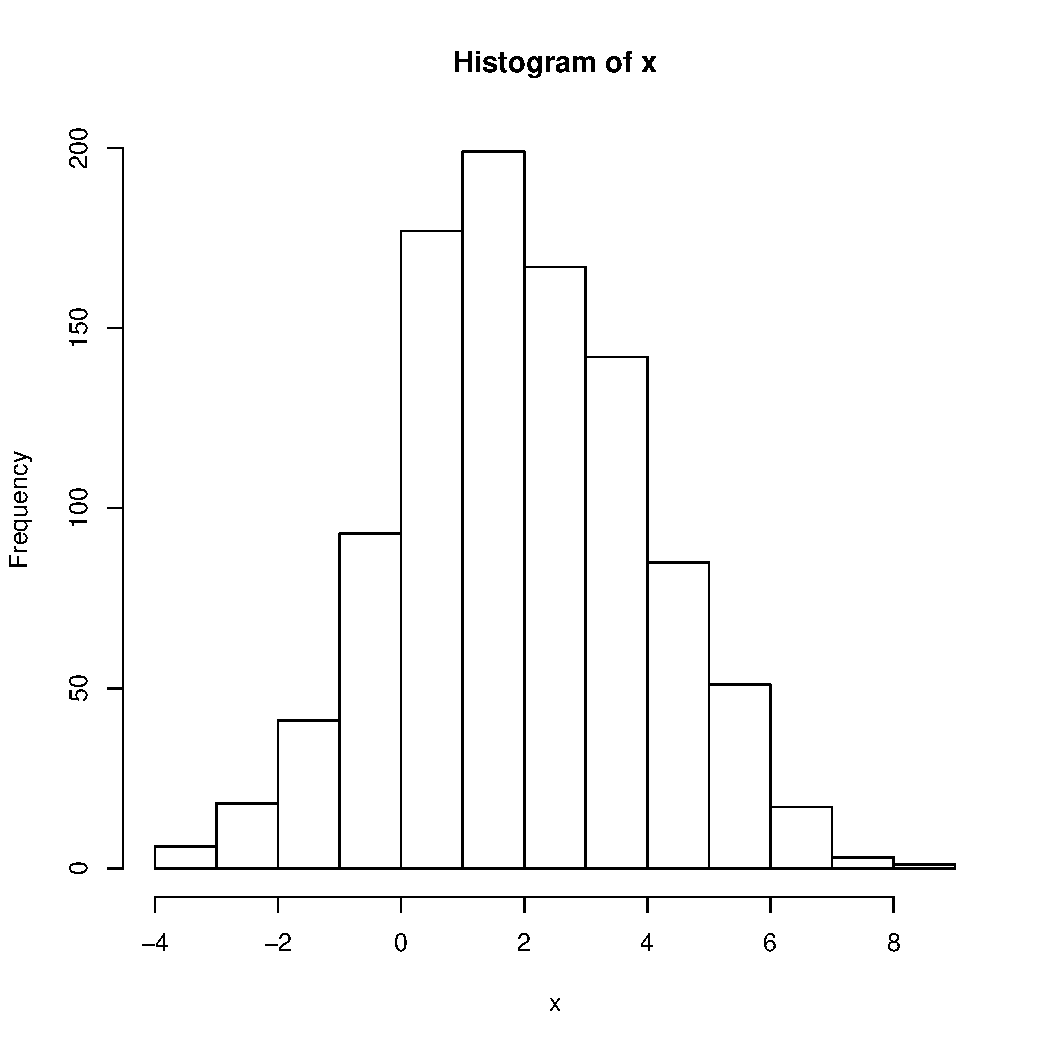
\includegraphics[width=\maxwidth]{figure/unnamed-chunk-17-1} 

\end{knitrout}
\medskip
\section{Vector manipulation.}
\subsection{Indexing vectors}
Extraction or replacement of parts of a vector can be performed using the "[" operator (which is equivalent to the \Rfunction{subset} function). Numeric vectors, logical vectors or names are used to indicate which positions in the vector are to be extracted or replaced.

\begin{knitrout}
\definecolor{shadecolor}{rgb}{0.969, 0.969, 0.969}\color{fgcolor}\begin{kframe}
\begin{alltt}
\hlkwd{set.seed}\hlstd{(}\hlnum{1}\hlstd{)}
\hlstd{x} \hlkwb{<-} \hlkwd{round}\hlstd{(}\hlkwd{rnorm}\hlstd{(}\hlnum{10}\hlstd{),}\hlnum{2}\hlstd{)}
\hlstd{x}
\end{alltt}
\begin{verbatim}
##  [1] -0.63  0.18 -0.84  1.60  0.33 -0.82  0.49  0.74  0.58 -0.31
\end{verbatim}
\begin{alltt}
\hlstd{x[}\hlnum{2}\hlstd{]}
\end{alltt}
\begin{verbatim}
## [1] 0.18
\end{verbatim}
\begin{alltt}
\hlstd{x[}\hlnum{1}\hlopt{:}\hlnum{3}\hlstd{]}
\end{alltt}
\begin{verbatim}
## [1] -0.63  0.18 -0.84
\end{verbatim}
\begin{alltt}
\hlstd{x[}\hlkwd{c}\hlstd{(}\hlnum{2}\hlstd{,}\hlnum{6}\hlstd{)]}
\end{alltt}
\begin{verbatim}
## [1]  0.18 -0.82
\end{verbatim}
\begin{alltt}
\hlkwd{which}\hlstd{(x}\hlopt{>}\hlnum{0}\hlstd{)}       \hlcom{# returns the positions containing positive values}
\end{alltt}
\begin{verbatim}
## [1] 2 4 5 7 8 9
\end{verbatim}
\begin{alltt}
\hlstd{x[}\hlkwd{which}\hlstd{(x}\hlopt{>}\hlnum{0}\hlstd{)]}    \hlcom{# returns the requested positive values (using a vector of integers)}
\end{alltt}
\begin{verbatim}
## [1] 0.18 1.60 0.33 0.49 0.74 0.58
\end{verbatim}
\begin{alltt}
\hlstd{x} \hlopt{>} \hlnum{0}            \hlcom{# returns TRUE if a positions contains a positive value}
\end{alltt}
\begin{verbatim}
##  [1] FALSE  TRUE FALSE  TRUE  TRUE FALSE  TRUE  TRUE  TRUE FALSE
\end{verbatim}
\begin{alltt}
\hlstd{x[x} \hlopt{>} \hlnum{0}\hlstd{]}
\end{alltt}
\begin{verbatim}
## [1] 0.18 1.60 0.33 0.49 0.74 0.58
\end{verbatim}
\begin{alltt}
\hlstd{nm} \hlkwb{<-} \hlkwd{paste}\hlstd{(}\hlstr{"n"}\hlstd{,}\hlnum{1}\hlopt{:}\hlnum{10}\hlstd{,} \hlkwc{sep}\hlstd{=}\hlstr{""}\hlstd{)}
\hlstd{nm}
\end{alltt}
\begin{verbatim}
##  [1] "n1"  "n2"  "n3"  "n4"  "n5"  "n6"  "n7"  "n8"  "n9"  "n10"
\end{verbatim}
\begin{alltt}
\hlkwd{names}\hlstd{(x)} \hlkwb{<-} \hlstd{nm}
\hlstd{x[}\hlstr{"n10"}\hlstd{]}          \hlcom{# Indexing with the names of the element}
\end{alltt}
\begin{verbatim}
##   n10 
## -0.31
\end{verbatim}
\end{kframe}
\end{knitrout}
\medskip



\subsection{Replacing parts of a vector}
Simply use the "<-" operators. Note that in R, missing values are defined as "NA" (Not Attributed).

\begin{knitrout}
\definecolor{shadecolor}{rgb}{0.969, 0.969, 0.969}\color{fgcolor}\begin{kframe}
\begin{alltt}
\hlstd{x[}\hlnum{1}\hlopt{:}\hlnum{2}\hlstd{]} \hlkwb{<-} \hlkwd{c}\hlstd{(}\hlnum{10}\hlstd{,}\hlnum{11}\hlstd{)}
\hlstd{x}
\end{alltt}
\begin{verbatim}
##    n1    n2    n3    n4    n5    n6    n7    n8    n9   n10 
## 10.00 11.00 -0.84  1.60  0.33 -0.82  0.49  0.74  0.58 -0.31
\end{verbatim}
\begin{alltt}
\hlstd{x[}\hlnum{4}\hlopt{:}\hlnum{6}\hlstd{]} \hlkwb{<-} \hlnum{NA}
\hlstd{x}
\end{alltt}
\begin{verbatim}
##    n1    n2    n3    n4    n5    n6    n7    n8    n9   n10 
## 10.00 11.00 -0.84    NA    NA    NA  0.49  0.74  0.58 -0.31
\end{verbatim}
\begin{alltt}
\hlkwd{is.na}\hlstd{(x)}              \hlcom{# returns TRUE if the position is NA}
\end{alltt}
\begin{verbatim}
##    n1    n2    n3    n4    n5    n6    n7    n8    n9   n10 
## FALSE FALSE FALSE  TRUE  TRUE  TRUE FALSE FALSE FALSE FALSE
\end{verbatim}
\begin{alltt}
\hlstd{x} \hlkwb{<-} \hlkwd{na.omit}\hlstd{(x)}       \hlcom{# To delete NA values}
\hlstd{x}
\end{alltt}
\begin{verbatim}
##    n1    n2    n3    n7    n8    n9   n10 
## 10.00 11.00 -0.84  0.49  0.74  0.58 -0.31 
## attr(,"na.action")
## n4 n5 n6 
##  4  5  6 
## attr(,"class")
## [1] "omit"
\end{verbatim}
\end{kframe}
\end{knitrout}
\medskip
\subsection{Vectorization}
R is intented to handle large data sets and to retrieve information using a concise syntax. Thanks to the internal feature of R, called \textit{vectorization}, numerous operation can be written without a loop:

\begin{knitrout}
\definecolor{shadecolor}{rgb}{0.969, 0.969, 0.969}\color{fgcolor}\begin{kframe}
\begin{alltt}
\hlstd{x} \hlkwb{<-} \hlnum{0}\hlopt{:}\hlnum{10}
\hlstd{y} \hlkwb{<-} \hlnum{20}\hlopt{:}\hlnum{30}
\hlstd{x}\hlopt{+}\hlstd{y}
\end{alltt}
\begin{verbatim}
##  [1] 20 22 24 26 28 30 32 34 36 38 40
\end{verbatim}
\begin{alltt}
\hlstd{x}\hlopt{^}\hlnum{2}
\end{alltt}
\begin{verbatim}
##  [1]   0   1   4   9  16  25  36  49  64  81 100
\end{verbatim}
\begin{alltt}
\hlkwd{sqrt}\hlstd{(x)}
\end{alltt}
\begin{verbatim}
##  [1] 0.000000 1.000000 1.414214 1.732051 2.000000 2.236068 2.449490
##  [8] 2.645751 2.828427 3.000000 3.162278
\end{verbatim}
\end{kframe}
\end{knitrout}
\medskip


\section{Objects of class: \Rfunction{factor}, \Rfunction{Matrix}, \Rfunction{data.frame} and \Rfunction{list}.}

\subsection{factor}
This object looks like a vector. It is used to store categorical variables. A vector can be converted to a factor using the \Rfunction{as.factor} function. The \Rfunction{levels} function can be used to extract the names of the categories and to rename them.

\begin{knitrout}
\definecolor{shadecolor}{rgb}{0.969, 0.969, 0.969}\color{fgcolor}\begin{kframe}
\begin{alltt}
\hlstd{x} \hlkwb{<-} \hlkwd{rep}\hlstd{(}\hlkwd{c}\hlstd{(}\hlstr{"good"}\hlstd{,}\hlstr{"bad"}\hlstd{),}\hlnum{5}\hlstd{)}
\hlstd{x}
\end{alltt}
\begin{verbatim}
##  [1] "good" "bad"  "good" "bad"  "good" "bad"  "good" "bad"  "good" "bad"
\end{verbatim}
\begin{alltt}
\hlstd{x} \hlkwb{<-} \hlkwd{as.factor}\hlstd{(x)}
\hlstd{x}
\end{alltt}
\begin{verbatim}
##  [1] good bad  good bad  good bad  good bad  good bad 
## Levels: bad good
\end{verbatim}
\begin{alltt}
\hlstd{x} \hlkwb{<-} \hlkwd{as.factor}\hlstd{(x)}
\hlstd{x}
\end{alltt}
\begin{verbatim}
##  [1] good bad  good bad  good bad  good bad  good bad 
## Levels: bad good
\end{verbatim}
\begin{alltt}
\hlkwd{levels}\hlstd{(x)}
\end{alltt}
\begin{verbatim}
## [1] "bad"  "good"
\end{verbatim}
\begin{alltt}
\hlkwd{levels}\hlstd{(x)} \hlkwb{<-} \hlnum{0}\hlopt{:}\hlnum{1}
\hlstd{x}
\end{alltt}
\begin{verbatim}
##  [1] 1 0 1 0 1 0 1 0 1 0
## Levels: 0 1
\end{verbatim}
\begin{alltt}
\hlkwd{table}\hlstd{(x)}
\end{alltt}
\begin{verbatim}
## x
## 0 1 
## 5 5
\end{verbatim}
\end{kframe}
\end{knitrout}
\medskip
\subsection{Matrix}
Matrix are intended to store 2-dimensional datasets. Each value will be of the same mode. As with vectors, one can use names, numeric vectors or a logical vector for indexing this object. One can index rows or columns or both.

\begin{knitrout}
\definecolor{shadecolor}{rgb}{0.969, 0.969, 0.969}\color{fgcolor}\begin{kframe}
\begin{alltt}
\hlstd{x} \hlkwb{<-} \hlkwd{matrix}\hlstd{(}\hlnum{1}\hlopt{:}\hlnum{10}\hlstd{,}\hlkwc{ncol}\hlstd{=}\hlnum{2}\hlstd{)}
\hlkwd{colnames}\hlstd{(x)} \hlkwb{<-} \hlkwd{c}\hlstd{(}\hlstr{"ctrl"}\hlstd{,}\hlstr{"trmt"}\hlstd{)}
\hlkwd{row.names}\hlstd{(x)} \hlkwb{<-} \hlkwd{paste}\hlstd{(}\hlstr{"gene"}\hlstd{,} \hlnum{1}\hlopt{:}\hlnum{5}\hlstd{,} \hlkwc{sep}\hlstd{=}\hlstr{"_"}\hlstd{)}
\hlstd{x}
\end{alltt}
\begin{verbatim}
##        ctrl trmt
## gene_1    1    6
## gene_2    2    7
## gene_3    3    8
## gene_4    4    9
## gene_5    5   10
\end{verbatim}
\begin{alltt}
\hlstd{x[,}\hlnum{1}\hlstd{]}                       \hlcom{# first column}
\end{alltt}
\begin{verbatim}
## gene_1 gene_2 gene_3 gene_4 gene_5 
##      1      2      3      4      5
\end{verbatim}
\begin{alltt}
\hlstd{x[}\hlnum{1}\hlstd{,]}                       \hlcom{# first row}
\end{alltt}
\begin{verbatim}
## ctrl trmt 
##    1    6
\end{verbatim}
\begin{alltt}
\hlstd{x[}\hlnum{1}\hlstd{,}\hlnum{2}\hlstd{]}                      \hlcom{# row 1 and column 2}
\end{alltt}
\begin{verbatim}
## [1] 6
\end{verbatim}
\begin{alltt}
\hlstd{x[}\hlkwd{c}\hlstd{(T,F,T,T,T),]}
\end{alltt}
\begin{verbatim}
##        ctrl trmt
## gene_1    1    6
## gene_3    3    8
## gene_4    4    9
## gene_5    5   10
\end{verbatim}
\end{kframe}
\end{knitrout}

Note that the syntax below that use a logical matrix is also frequently used to extract or replace part of a matrix.

\begin{knitrout}
\definecolor{shadecolor}{rgb}{0.969, 0.969, 0.969}\color{fgcolor}\begin{kframe}
\begin{alltt}
\hlstd{x} \hlopt{<} \hlnum{2} \hlopt{|} \hlstd{x} \hlopt{>} \hlnum{8}
\end{alltt}
\begin{verbatim}
##         ctrl  trmt
## gene_1  TRUE FALSE
## gene_2 FALSE FALSE
## gene_3 FALSE FALSE
## gene_4 FALSE  TRUE
## gene_5 FALSE  TRUE
\end{verbatim}
\begin{alltt}
\hlstd{x[x} \hlopt{<} \hlnum{2} \hlopt{|} \hlstd{x} \hlopt{>} \hlnum{8}\hlstd{]} \hlkwb{<-}  \hlnum{NA}
\end{alltt}
\end{kframe}
\end{knitrout}


\subsection{data.frame}
This object is very similar to the matrix except that each column can contain a given mode (a column with characters, a column with logicals, a column with numerics,...).

\subsection{list}
Object of class list can store any type of object. They should be indexed with the "[[" or \$ operators.

\begin{knitrout}
\definecolor{shadecolor}{rgb}{0.969, 0.969, 0.969}\color{fgcolor}\begin{kframe}
\begin{alltt}
\hlstd{l1} \hlkwb{<-} \hlkwd{list}\hlstd{(}\hlkwc{A}\hlstd{=x,} \hlkwc{B}\hlstd{=}\hlkwd{rnorm}\hlstd{(}\hlnum{10}\hlstd{))}
\hlstd{l1}
\end{alltt}
\begin{verbatim}
## $A
##        ctrl trmt
## gene_1   NA    6
## gene_2    2    7
## gene_3    3    8
## gene_4    4   NA
## gene_5    5   NA
## 
## $B
##  [1]  1.51178117  0.38984324 -0.62124058 -2.21469989  1.12493092
##  [6] -0.04493361 -0.01619026  0.94383621  0.82122120  0.59390132
\end{verbatim}
\begin{alltt}
\hlkwd{is}\hlstd{(l1[[}\hlnum{1}\hlstd{]])}
\end{alltt}
\begin{verbatim}
## [1] "matrix"    "array"     "structure" "vector"
\end{verbatim}
\begin{alltt}
\hlkwd{is}\hlstd{(l1[[}\hlnum{2}\hlstd{]])}
\end{alltt}
\begin{verbatim}
## [1] "numeric" "vector"
\end{verbatim}
\begin{alltt}
\hlstd{l1}\hlopt{$}\hlstd{A}
\end{alltt}
\begin{verbatim}
##        ctrl trmt
## gene_1   NA    6
## gene_2    2    7
## gene_3    3    8
## gene_4    4   NA
## gene_5    5   NA
\end{verbatim}
\end{kframe}
\end{knitrout}


\subsection{The "Apply" family of functions}

They are used to loop through row and columns of a matrix (or dataframe) or through elements of a list.

\susection{The \Rfunction{apply} function}
\begin{knitrout}
\definecolor{shadecolor}{rgb}{0.969, 0.969, 0.969}\color{fgcolor}\begin{kframe}
\begin{alltt}
\hlstd{x} \hlkwb{<-} \hlkwd{matrix}\hlstd{(}\hlnum{1}\hlopt{:}\hlnum{10}\hlstd{,}\hlkwc{ncol}\hlstd{=}\hlnum{2}\hlstd{)}
\hlkwd{apply}\hlstd{(x,}\hlnum{1}\hlstd{, sd)}        \hlcom{# 1 stands for rows}
\end{alltt}
\begin{verbatim}
## [1] 3.535534 3.535534 3.535534 3.535534 3.535534
\end{verbatim}
\begin{alltt}
\hlkwd{apply}\hlstd{(x,}\hlnum{2}\hlstd{, sd)}        \hlcom{# 2 stands for colums}
\end{alltt}
\begin{verbatim}
## [1] 1.581139 1.581139
\end{verbatim}
\end{kframe}
\end{knitrout}

\susection{The \Rfunction{lapply} function}
The \Rfunction{\textbf{l}apply} is used for \textbf{l}ist (or data.frame).

\begin{knitrout}
\definecolor{shadecolor}{rgb}{0.969, 0.969, 0.969}\color{fgcolor}\begin{kframe}
\begin{alltt}
\hlkwd{lapply}\hlstd{(l1, is)}        \hlcom{# The types of the object stored in the list.}
\end{alltt}
\begin{verbatim}
## $A
## [1] "matrix"    "array"     "structure" "vector"   
## 
## $B
## [1] "numeric" "vector"
\end{verbatim}
\end{kframe}
\end{knitrout}


\subsection{The \Rfunction{tapply} function}
This function tipically takes a vector and a factor as arguments. For instance, we have data that fall in three caterogies ("good", "bad", "medium"). We can compute different statistics related to the category:

\begin{knitrout}
\definecolor{shadecolor}{rgb}{0.969, 0.969, 0.969}\color{fgcolor}\begin{kframe}
\begin{alltt}
\hlstd{cat} \hlkwb{<-} \hlkwd{rep}\hlstd{(}\hlkwd{c}\hlstd{(}\hlstr{"good"}\hlstd{,} \hlstr{"bad"}\hlstd{,} \hlstr{"medium"}\hlstd{),}\hlnum{5}\hlstd{)}
\hlstd{cat} \hlkwb{<-} \hlkwd{as.factor}\hlstd{(cat)}
\hlstd{x} \hlkwb{<-} \hlkwd{rnorm}\hlstd{(}\hlkwd{length}\hlstd{(cat))}
\hlstd{x[cat} \hlopt{==} \hlstr{"good"}\hlstd{]} \hlkwb{<-} \hlstd{x[cat} \hlopt{==} \hlstr{"good"}\hlstd{]}\hlopt{+}\hlnum{2}
\hlstd{x[cat} \hlopt{==} \hlstr{"medium"}\hlstd{]} \hlkwb{<-} \hlstd{x[cat} \hlopt{==} \hlstr{"medium"}\hlstd{]}\hlopt{+}\hlnum{1}
\hlkwd{boxplot}\hlstd{(x}\hlopt{~}\hlstd{cat)}
\end{alltt}
\end{kframe}
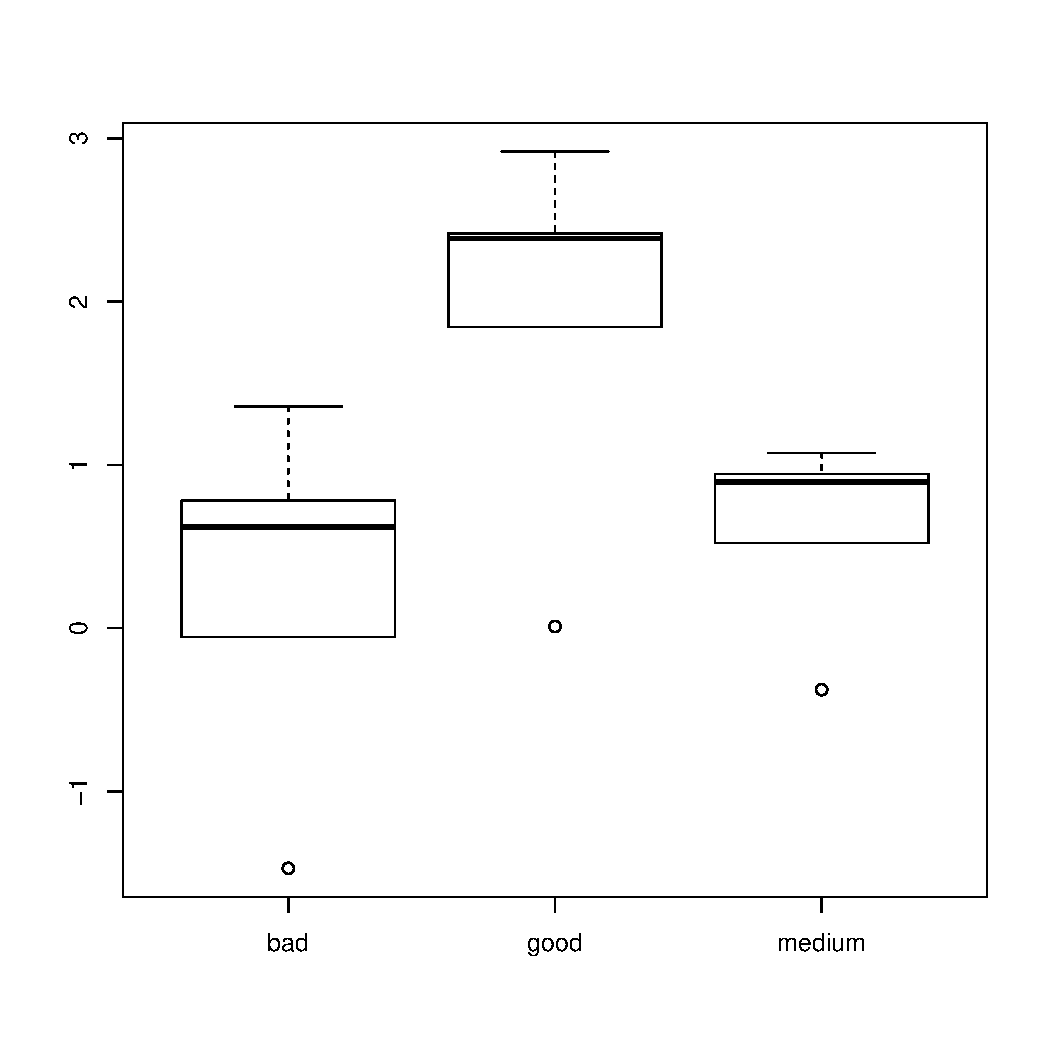
\includegraphics[width=\maxwidth]{figure/unnamed-chunk-27-1} 
\begin{kframe}\begin{alltt}
\hlkwd{tapply}\hlstd{(x,cat,sd)}
\end{alltt}
\begin{verbatim}
##       bad      good    medium 
## 1.0842461 1.1309181 0.5898764
\end{verbatim}
\begin{alltt}
\hlkwd{tapply}\hlstd{(x,cat,mean)}
\end{alltt}
\begin{verbatim}
##       bad      good    medium 
## 0.2472168 1.9158887 0.6120878
\end{verbatim}
\begin{alltt}
\hlkwd{tapply}\hlstd{(x,cat,length)}
\end{alltt}
\begin{verbatim}
##    bad   good medium 
##      5      5      5
\end{verbatim}
\end{kframe}
\end{knitrout}


\subsection{Graphics with R}

\subsection{Graphics}

R offers a large variety of high-level graphics functions (\Rfunction{plot}, \Rfunction{boxplot}, \Rfunction{barplot}, \Rfunction{hist}, \Rfunction{pairs}, \Rfunction{image}, ...). The generated graphics can be modified using low-level functions (\textbf{points}, \textbf{text}, \textbf{line}, \textbf{abline}, \textbf{rect}, \textbf{legend}, ...).

\subsection{A simple example using two colour microarray data processed with basic R functions.}

\paragraph{Loading and visualizing the data}
\begin{knitrout}
\definecolor{shadecolor}{rgb}{0.969, 0.969, 0.969}\color{fgcolor}\begin{kframe}
\begin{alltt}
\hlcom{# Create an OS-independent path to the directory "swirldata"}
\hlcom{# located in the package "marray"}
\hlstd{path} \hlkwb{<-} \hlkwd{system.file}\hlstd{(}\hlstr{"swirldata"}\hlstd{,} \hlkwc{package} \hlstd{=} \hlstr{"marray"}\hlstd{)}
\hlstd{path}
\end{alltt}
\begin{verbatim}
## [1] ""
\end{verbatim}
\begin{alltt}
\hlkwd{getwd}\hlstd{()}                   \hlcom{# the current working directory}
\end{alltt}
\begin{verbatim}
## [1] "/Users/jvanheld/Documents/enseignement/bioinformatics_courses/ASG1/practicals/r_intro_en"
\end{verbatim}
\begin{alltt}
\hlkwd{setwd}\hlstd{(path)}               \hlcom{# set working directory to "path"}
\end{alltt}


{\ttfamily\noindent\bfseries\color{errorcolor}{\#\# Error in setwd(path): cannot change working directory}}\begin{alltt}
\hlkwd{getwd}\hlstd{()}                   \hlcom{# The working directory has changed}
\end{alltt}
\begin{verbatim}
## [1] "/Users/jvanheld/Documents/enseignement/bioinformatics_courses/ASG1/practicals/r_intro_en"
\end{verbatim}
\begin{alltt}
\hlkwd{dir}\hlstd{()}                     \hlcom{# list the working directory}
\end{alltt}
\begin{verbatim}
##  [1] "figure"                    "Rplots.pdf"               
##  [3] "RQuickTutorial"            "RQuickTutorial.dvi"       
##  [5] "RQuickTutorial.html"       "RQuickTutorial.pdf"       
##  [7] "RQuickTutorial.R"          "RQuickTutorial.Rnw"       
##  [9] "RQuickTutorial.Rnw.backup" "RQuickTutorial.tex"       
## [11] "RQuickTutorial.toc"        "sweave2html.sh"
\end{verbatim}
\begin{alltt}
\hlcom{#file.show("swirl.1.spot") # this file contains a Header}
\hlstd{d} \hlkwb{<-} \hlkwd{read.table}\hlstd{(}\hlstr{"swirl.1.spot"}\hlstd{,} \hlkwc{header}\hlstd{=T,} \hlkwc{sep}\hlstd{=}\hlstr{"\textbackslash{}t"}\hlstd{,} \hlkwc{row.names}\hlstd{=}\hlnum{1}\hlstd{)}
\end{alltt}


{\ttfamily\noindent\color{warningcolor}{\#\# Warning in file(file, "{}rt"{}): cannot open file 'swirl.1.spot': No such file or directory}}

{\ttfamily\noindent\bfseries\color{errorcolor}{\#\# Error in file(file, "{}rt"{}): cannot open the connection}}\begin{alltt}
\hlkwd{is}\hlstd{(d)}
\end{alltt}


{\ttfamily\noindent\bfseries\color{errorcolor}{\#\# Error in is(d): object 'd' not found}}\begin{alltt}
\hlkwd{colnames}\hlstd{(d)}
\end{alltt}


{\ttfamily\noindent\bfseries\color{errorcolor}{\#\# Error in is.data.frame(x): object 'd' not found}}\begin{alltt}
\hlstd{G} \hlkwb{<-} \hlstd{d[,}\hlstr{"Gmedian"}\hlstd{]}
\end{alltt}


{\ttfamily\noindent\bfseries\color{errorcolor}{\#\# Error in eval(expr, envir, enclos): object 'd' not found}}\begin{alltt}
\hlstd{R} \hlkwb{<-} \hlstd{d[,}\hlstr{"Rmedian"}\hlstd{]}
\end{alltt}


{\ttfamily\noindent\bfseries\color{errorcolor}{\#\# Error in eval(expr, envir, enclos): object 'd' not found}}\begin{alltt}
\hlkwd{plot}\hlstd{(R,G,} \hlkwc{pch}\hlstd{=}\hlnum{16}\hlstd{,} \hlkwc{cex}\hlstd{=}\hlnum{0.5}\hlstd{,} \hlkwc{col}\hlstd{=}\hlstr{"red"}\hlstd{)} \hlcom{# low values are densely packed}
\end{alltt}


{\ttfamily\noindent\bfseries\color{errorcolor}{\#\# Error in plot(R, G, pch = 16, cex = 0.5, col = "{}red"{}): object 'R' not found}}\begin{alltt}
                                      \hlcom{# in the UL corner}
\hlkwd{library}\hlstd{(geneplotter)}
\end{alltt}


{\ttfamily\noindent\bfseries\color{errorcolor}{\#\# Error in library(geneplotter): there is no package called 'geneplotter'}}\begin{alltt}
\hlkwd{smoothScatter}\hlstd{(R,G)}                    \hlcom{# even more marked}
\end{alltt}


{\ttfamily\noindent\bfseries\color{errorcolor}{\#\# Error in xy.coords(x, y, xlabel, ylabel): object 'G' not found}}\begin{alltt}
\hlkwd{boxplot}\hlstd{(R,G)}                          \hlcom{# 1rst , 2nd (median) and 3rd quartile}
\end{alltt}


{\ttfamily\noindent\bfseries\color{errorcolor}{\#\# Error in boxplot(R, G): object 'R' not found}}\begin{alltt}
\hlstd{R} \hlkwb{<-} \hlkwd{log2}\hlstd{(R)}
\end{alltt}


{\ttfamily\noindent\bfseries\color{errorcolor}{\#\# Error in eval(expr, envir, enclos): object 'R' not found}}\begin{alltt}
\hlstd{G} \hlkwb{<-} \hlkwd{log2}\hlstd{(G)}
\end{alltt}


{\ttfamily\noindent\bfseries\color{errorcolor}{\#\# Error in eval(expr, envir, enclos): object 'G' not found}}\begin{alltt}
\hlkwd{plot}\hlstd{(R,G,} \hlkwc{pch}\hlstd{=}\hlnum{16}\hlstd{,} \hlkwc{cex}\hlstd{=}\hlnum{0.5}\hlstd{,} \hlkwc{col}\hlstd{=}\hlstr{"red"}\hlstd{)}
\end{alltt}


{\ttfamily\noindent\bfseries\color{errorcolor}{\#\# Error in plot(R, G, pch = 16, cex = 0.5, col = "{}red"{}): object 'R' not found}}\begin{alltt}
\hlkwd{boxplot}\hlstd{(R,G)}
\end{alltt}


{\ttfamily\noindent\bfseries\color{errorcolor}{\#\# Error in boxplot(R, G): object 'R' not found}}\end{kframe}
\end{knitrout}

\paragraph{MA plot}
A MA plot without normalization.
\begin{knitrout}
\definecolor{shadecolor}{rgb}{0.969, 0.969, 0.969}\color{fgcolor}\begin{kframe}
\begin{alltt}
\hlstd{M} \hlkwb{<-} \hlstd{R}\hlopt{-}\hlstd{G}
\end{alltt}


{\ttfamily\noindent\bfseries\color{errorcolor}{\#\# Error in eval(expr, envir, enclos): object 'R' not found}}\begin{alltt}
\hlstd{A} \hlkwb{<-} \hlstd{R}\hlopt{+}\hlstd{G}
\end{alltt}


{\ttfamily\noindent\bfseries\color{errorcolor}{\#\# Error in eval(expr, envir, enclos): object 'R' not found}}\begin{alltt}
\hlkwd{plot}\hlstd{(A,M,} \hlkwc{pch}\hlstd{=}\hlnum{16}\hlstd{,}\hlkwc{cex} \hlstd{=}\hlnum{0.5}\hlstd{)}
\end{alltt}


{\ttfamily\noindent\bfseries\color{errorcolor}{\#\# Error in plot(A, M, pch = 16, cex = 0.5): object 'A' not found}}\begin{alltt}
\hlstd{low} \hlkwb{<-} \hlkwd{lowess}\hlstd{(M}\hlopt{~}\hlstd{A)}
\end{alltt}


{\ttfamily\noindent\bfseries\color{errorcolor}{\#\# Error in eval(expr, envir, enclos): object 'M' not found}}\begin{alltt}
\hlkwd{lines}\hlstd{(low,}\hlkwc{col}\hlstd{=}\hlstr{"blue"}\hlstd{,} \hlkwc{lwd} \hlstd{=} \hlnum{2}\hlstd{)}       \hlcom{# lwd: line width}
\end{alltt}


{\ttfamily\noindent\bfseries\color{errorcolor}{\#\# Error in lines(low, col = "{}blue"{}, lwd = 2): object 'low' not found}}\begin{alltt}
\hlkwd{abline}\hlstd{(}\hlkwc{h}\hlstd{=}\hlnum{0}\hlstd{,} \hlkwc{col}\hlstd{=}\hlstr{"red"}\hlstd{)}              \hlcom{# h: horizontal}
\end{alltt}


{\ttfamily\noindent\bfseries\color{errorcolor}{\#\# Error in int\_abline(a = a, b = b, h = h, v = v, untf = untf, ...): plot.new has not been called yet}}\begin{alltt}
\hlkwd{abline}\hlstd{(}\hlkwc{h}\hlstd{=}\hlopt{-}\hlnum{1}\hlstd{,} \hlkwc{col}\hlstd{=}\hlstr{"green"}\hlstd{)}
\end{alltt}


{\ttfamily\noindent\bfseries\color{errorcolor}{\#\# Error in int\_abline(a = a, b = b, h = h, v = v, untf = untf, ...): plot.new has not been called yet}}\begin{alltt}
\hlkwd{abline}\hlstd{(}\hlkwc{h}\hlstd{=}\hlnum{1}\hlstd{,} \hlkwc{col}\hlstd{=}\hlstr{"green"}\hlstd{)}
\end{alltt}


{\ttfamily\noindent\bfseries\color{errorcolor}{\#\# Error in int\_abline(a = a, b = b, h = h, v = v, untf = untf, ...): plot.new has not been called yet}}\begin{alltt}
\hlcom{# Genes considered as "good" have an}
\hlcom{# absolute ratio of 1 (2 in linear scale).}
\hlstd{good} \hlkwb{<-} \hlkwd{abs}\hlstd{(M)} \hlopt{>} \hlnum{1}
\end{alltt}


{\ttfamily\noindent\bfseries\color{errorcolor}{\#\# Error in eval(expr, envir, enclos): object 'M' not found}}\begin{alltt}
\hlkwd{points}\hlstd{(A[good], M[good],} \hlkwc{col}\hlstd{=}\hlstr{"red"}\hlstd{)}
\end{alltt}


{\ttfamily\noindent\bfseries\color{errorcolor}{\#\# Error in points(A[good], M[good], col = "{}red"{}): object 'A' not found}}\begin{alltt}
\hlcom{# They aren't so good...}
\hlstd{gn} \hlkwb{<-} \hlnum{1}\hlopt{:}\hlkwd{nrow}\hlstd{(d)}
\end{alltt}


{\ttfamily\noindent\bfseries\color{errorcolor}{\#\# Error in nrow(d): object 'd' not found}}\begin{alltt}
\hlkwd{text}\hlstd{(A[good], M[good],} \hlkwc{lab}\hlstd{=gn[good],}\hlkwc{cex}\hlstd{=}\hlnum{0.4}\hlstd{,}\hlkwc{pos}\hlstd{=}\hlnum{2}\hlstd{)}
\end{alltt}


{\ttfamily\noindent\bfseries\color{errorcolor}{\#\# Error in text(A[good], M[good], lab = gn[good], cex = 0.4, pos = 2): object 'A' not found}}\end{kframe}
\end{knitrout}


\subsection{S4 objects in R}
In the last example, we have used Gmedian and  Rmedian data. However, we should have also considered the background signal. The problem is that we should have created four vectors (or four matrix if several microarrays were analyzed). As it is rather difficult to manipulate the four matrices we will design a class ("micBatch") that will contain all information within a single object.

\begin{knitrout}
\definecolor{shadecolor}{rgb}{0.969, 0.969, 0.969}\color{fgcolor}\begin{kframe}
\begin{alltt}
\hlcom{# micBatch}
\hlcom{# "representation" corresponds to all attributes of the object:}
\hlcom{# "prototype" corresponds corresponds to default values:}

\hlkwd{setClass}\hlstd{(}\hlstr{"micBatch"}\hlstd{,}
    \hlkwd{representation}\hlstd{(}
        \hlkwc{R}\hlstd{=}\hlstr{"matrix"}\hlstd{,}
        \hlkwc{G}\hlstd{=}\hlstr{"matrix"}\hlstd{,}
        \hlkwc{Rb}\hlstd{=}\hlstr{"matrix"}\hlstd{,}
        \hlkwc{Gb}\hlstd{=}\hlstr{"matrix"}\hlstd{,}
        \hlkwc{phenotype}\hlstd{=}\hlstr{"matrix"}\hlstd{,}
        \hlkwc{genes}\hlstd{=}\hlstr{"character"}\hlstd{,}
        \hlkwc{description}\hlstd{=}\hlstr{"character"}\hlstd{),}
    \hlkwc{prototype}\hlstd{=}\hlkwd{list}\hlstd{(}
        \hlkwc{R}\hlstd{=}\hlkwd{matrix}\hlstd{(}\hlkwc{nr}\hlstd{=}\hlnum{0}\hlstd{,}\hlkwc{nc}\hlstd{=}\hlnum{0}\hlstd{),}
        \hlkwc{G}\hlstd{=}\hlkwd{matrix}\hlstd{(}\hlkwc{nr}\hlstd{=}\hlnum{0}\hlstd{,}\hlkwc{nc}\hlstd{=}\hlnum{0}\hlstd{),}
        \hlkwc{Rb}\hlstd{=}\hlkwd{matrix}\hlstd{(}\hlkwc{nr}\hlstd{=}\hlnum{0}\hlstd{,}\hlkwc{nc}\hlstd{=}\hlnum{0}\hlstd{),}
        \hlkwc{Gb}\hlstd{=}\hlkwd{matrix}\hlstd{(}\hlkwc{nr}\hlstd{=}\hlnum{0}\hlstd{,}\hlkwc{nc}\hlstd{=}\hlnum{0}\hlstd{),}
        \hlkwc{phenotype}\hlstd{=}\hlkwd{matrix}\hlstd{(}\hlkwc{nr}\hlstd{=}\hlnum{0}\hlstd{,}\hlkwc{nc}\hlstd{=}\hlnum{0}\hlstd{),}
        \hlkwc{description}\hlstd{=}\hlkwd{new}\hlstd{(}\hlstr{"character"}\hlstd{)}
            \hlstd{)}
    \hlstd{)}

\hlstd{myMA}\hlkwb{=}\hlkwd{new}\hlstd{(}\hlstr{"micBatch"}\hlstd{)}

\hlkwd{slotNames}\hlstd{(myMA)}
\end{alltt}
\begin{verbatim}
## [1] "R"           "G"           "Rb"          "Gb"          "phenotype"  
## [6] "genes"       "description"
\end{verbatim}
\begin{alltt}
\hlkwd{getClassDef}\hlstd{(}\hlstr{"micBatch"}\hlstd{)}
\end{alltt}
\begin{verbatim}
## Class "micBatch" [in ".GlobalEnv"]
## 
## Slots:
##                                                                   
## Name:            R           G          Rb          Gb   phenotype
## Class:      matrix      matrix      matrix      matrix      matrix
##                               
## Name:        genes description
## Class:   character   character
\end{verbatim}
\begin{alltt}
\hlstd{myMA}\hlopt{@}\hlkwc{R} \hlkwb{<-} \hlkwd{matrix}\hlstd{(}\hlkwd{rnorm}\hlstd{(}\hlnum{20}\hlstd{),}\hlkwc{nc}\hlstd{=}\hlnum{5}\hlstd{)}
\hlstd{myMA}\hlopt{@}\hlkwc{R} \hlkwb{<-} \hlkwd{matrix}\hlstd{(}\hlkwd{rnorm}\hlstd{(}\hlnum{20}\hlstd{),}\hlkwc{nc}\hlstd{=}\hlnum{5}\hlstd{)}
\hlstd{myMA}\hlopt{@}\hlkwc{Rb} \hlkwb{<-} \hlkwd{matrix}\hlstd{(}\hlkwd{rnorm}\hlstd{(}\hlnum{20}\hlstd{),}\hlkwc{nc}\hlstd{=}\hlnum{5}\hlstd{)}
\hlstd{myMA}\hlopt{@}\hlkwc{Gb} \hlkwb{<-} \hlkwd{matrix}\hlstd{(}\hlkwd{rnorm}\hlstd{(}\hlnum{20}\hlstd{),}\hlkwc{nc}\hlstd{=}\hlnum{5}\hlstd{)}

\hlcom{# let's visualize the object.}
\hlcom{# (implicit call to the "show" method).}
\hlstd{myMA}
\end{alltt}
\begin{verbatim}
## An object of class "micBatch"
## Slot "R":
##            [,1]       [,2]        [,3]      [,4]       [,5]
## [1,]  1.9803999 -0.1350546  0.02800216 1.4655549 -0.7099464
## [2,] -0.3672215  2.4016178 -0.74327321 0.1532533  0.6107264
## [3,] -1.0441346 -0.0392400  0.18879230 2.1726117 -0.9340976
## [4,]  0.5697196  0.6897394 -1.80495863 0.4755095 -1.2536334
## 
## Slot "G":
## <0 x 0 matrix>
## 
## Slot "Rb":
##              [,1]       [,2]       [,3]       [,4]      [,5]
## [1,]  0.291446236 -0.5895209 -1.5235668 -0.3041839 1.2078678
## [2,] -0.443291873 -0.5686687  0.5939462  0.3700188 1.1604026
## [3,]  0.001105352 -0.1351786  0.3329504  0.2670988 0.7002136
## [4,]  0.074341324  1.1780870  1.0630998 -0.5425200 1.5868335
## 
## Slot "Gb":
##            [,1]        [,2]       [,3]       [,4]       [,5]
## [1,]  0.5584864 -0.47340064  0.1580288  0.9101742 -0.4616447
## [2,] -1.2765922 -0.62036668 -0.6545846  0.3841854  1.4322822
## [3,] -0.5732654  0.04211587  1.7672873  1.6821761 -0.6506964
## [4,] -1.2246126 -0.91092165  0.7167075 -0.6357365 -0.2073807
## 
## Slot "phenotype":
## <0 x 0 matrix>
## 
## Slot "genes":
## character(0)
## 
## Slot "description":
## character(0)
\end{verbatim}
\begin{alltt}
\hlcom{# Let's define the method "show" for an object of class}
\hlcom{# micBatch}

\hlkwd{setMethod}\hlstd{(}\hlstr{"show"}\hlstd{,} \hlkwd{signature}\hlstd{(}\hlstr{"micBatch"}\hlstd{),}
       \hlkwa{function}\hlstd{(}\hlkwc{object}\hlstd{)\{}
        \hlkwd{cat}\hlstd{(}\hlstr{"An instance of class micBatch\textbackslash{}n"}\hlstd{)}
        \hlkwd{cat}\hlstd{(}\hlstr{"Nb sample="}\hlstd{,} \hlkwd{ncol}\hlstd{(object}\hlopt{@}\hlkwc{R}\hlstd{),}\hlstr{"\textbackslash{}n"}\hlstd{)}
        \hlkwd{cat}\hlstd{(}\hlstr{"Nb genes="}\hlstd{,} \hlkwd{nrow}\hlstd{(object}\hlopt{@}\hlkwc{R}\hlstd{),}\hlstr{"\textbackslash{}n"}\hlstd{)}
\hlstd{\})}
\end{alltt}
\begin{verbatim}
## [1] "show"
\end{verbatim}
\begin{alltt}
\hlcom{# Let's call the "show" method}
\hlstd{myMA}
\end{alltt}
\begin{verbatim}
## An instance of class micBatch
## Nb sample= 5 
## Nb genes= 4
\end{verbatim}
\end{kframe}
\end{knitrout}

As shown in this example we can easily define methods for the class \Rfunction{micBatch}. Just remind that we could have define a method for the "[" operator. This would have been particularly interesting to extract rows (genes) and columns (arrays) of the object.


\section{Bioconductor}
Bioconductor offers a set of libraries of functions that are useful to biologists (see http://bioconductor.org for more informations)


\begin{itemize}
\item cDNA Microarray analysis:\\
  -marray, ArrayQuality, arrayMagic, limma, sma
\item  Affymetrix GeneChip analysis:\\
  -Affy, simpleaffy
\item  Probe Metadata:\\
- Annotate, hgu133aprobe,  hgu95av2probe, ABPkgBuilder
\item High level plotting functions
- geneplotter
\item  Microarray data filtering:\\
  -Genefilter
\item  Statistical analysis:\\
  -SAMR, siggenes, multtest, DEDS, pickgene
\item Interpretation:\\
  -GO, Gostats, goCluster, geneplotter
\item Graphs:\\
  -graph, Rgraphviz, biocGraph,
\item Training datasets:\\
  -golubEsets, fibroEseT...
\item Flow cytometry:\\
  -flowCore, flowViZ...
\item Proteomics
  -MassSpecWavelet, PROcess, xcms...
\item Image analysis:\\
  -EBImage
\end{itemize}


\subsection{Example: 2 color Arrays}

Affymetrix data can be analyzed using the \Rfunction{affy} package.\\
You can run this example using raw data of the GSE2004 dataset (Gene Expression Omnibus).\\

\begin{knitrout}
\definecolor{shadecolor}{rgb}{0.969, 0.969, 0.969}\color{fgcolor}\begin{kframe}
\begin{alltt}
\hlkwd{library}\hlstd{(marray)}
\hlstd{path} \hlkwb{<-} \hlkwd{system.file}\hlstd{(}\hlstr{"swirldata"}\hlstd{,} \hlkwc{package} \hlstd{=} \hlstr{"marray"}\hlstd{)}
\hlkwd{setwd}\hlstd{(path)}
\hlstd{m} \hlkwb{<-} \hlkwd{read.Spot}\hlstd{()}
\hlkwd{plot}\hlstd{(m[,}\hlnum{1}\hlstd{])}
\hlkwd{maImage}\hlstd{(m[,}\hlnum{1}\hlstd{])}
\hlstd{n} \hlkwb{<-} \hlkwd{maNorm}\hlstd{(m,}\hlkwc{norm}\hlstd{=}\hlstr{"printTipLoess"}\hlstd{)}
\hlkwd{plot}\hlstd{(n[,}\hlnum{1}\hlstd{])}
\hlkwd{plot}\hlstd{(n[,}\hlnum{2}\hlstd{])}
\end{alltt}
\end{kframe}
\end{knitrout}


\subsection{Example: Affy Data normalization}

Affymetrix data can be analyzed using the \Rfunction{affy} package.\\
You can run this example using raw data of the GSE2004 dataset (Gene Expression Omnibus).\\

\begin{knitrout}
\definecolor{shadecolor}{rgb}{0.969, 0.969, 0.969}\color{fgcolor}\begin{kframe}
\begin{alltt}
\hlkwd{setwd}\hlstd{(}\hlstr{"/where/the/cel/files/are"}\hlstd{)}
\hlkwd{library}\hlstd{(affy)}
\hlstd{d} \hlkwb{<-} \hlkwd{ReadAffy}\hlstd{()}
\hlkwd{is}\hlstd{(d)}
\hlkwd{image}\hlstd{(d[,}\hlnum{1}\hlstd{])}
\hlstd{n} \hlkwb{<-} \hlkwd{rma}\hlstd{(d)}
\hlkwd{write.exprs}\hlstd{(n,}\hlstr{"normalized.txt"}\hlstd{)}
\end{alltt}
\end{kframe}
\end{knitrout}

\section{Further readings}
\begin{itemize}
 \item R for beginners\\
 http://cran.r-project.org/doc/contrib/Paradis-rdebuts\_en.pdf\\
 \item Bioinformatics and Computational Biology Solutions Using R and Bioconductor. Robert Gentleman, Vincent Carey, Wolfgang Huber, Rafael Irizarry, Sandrine Dudoit.ISBN: 978-0-387-25146-2\\.
 http://www.springer.com/computer/computational+biology+and+bioinformatics/book/978-0-387-25146-2

\end{itemize}


\end{document}
